%\vspace{-4pt}
\subsection{Overview}
\label{sec:overview}
%\vspace{-4pt}

\begin{figure*}[t]
	\centering
		%\begin{minipage}{0.225\textwidth}
			\centering
			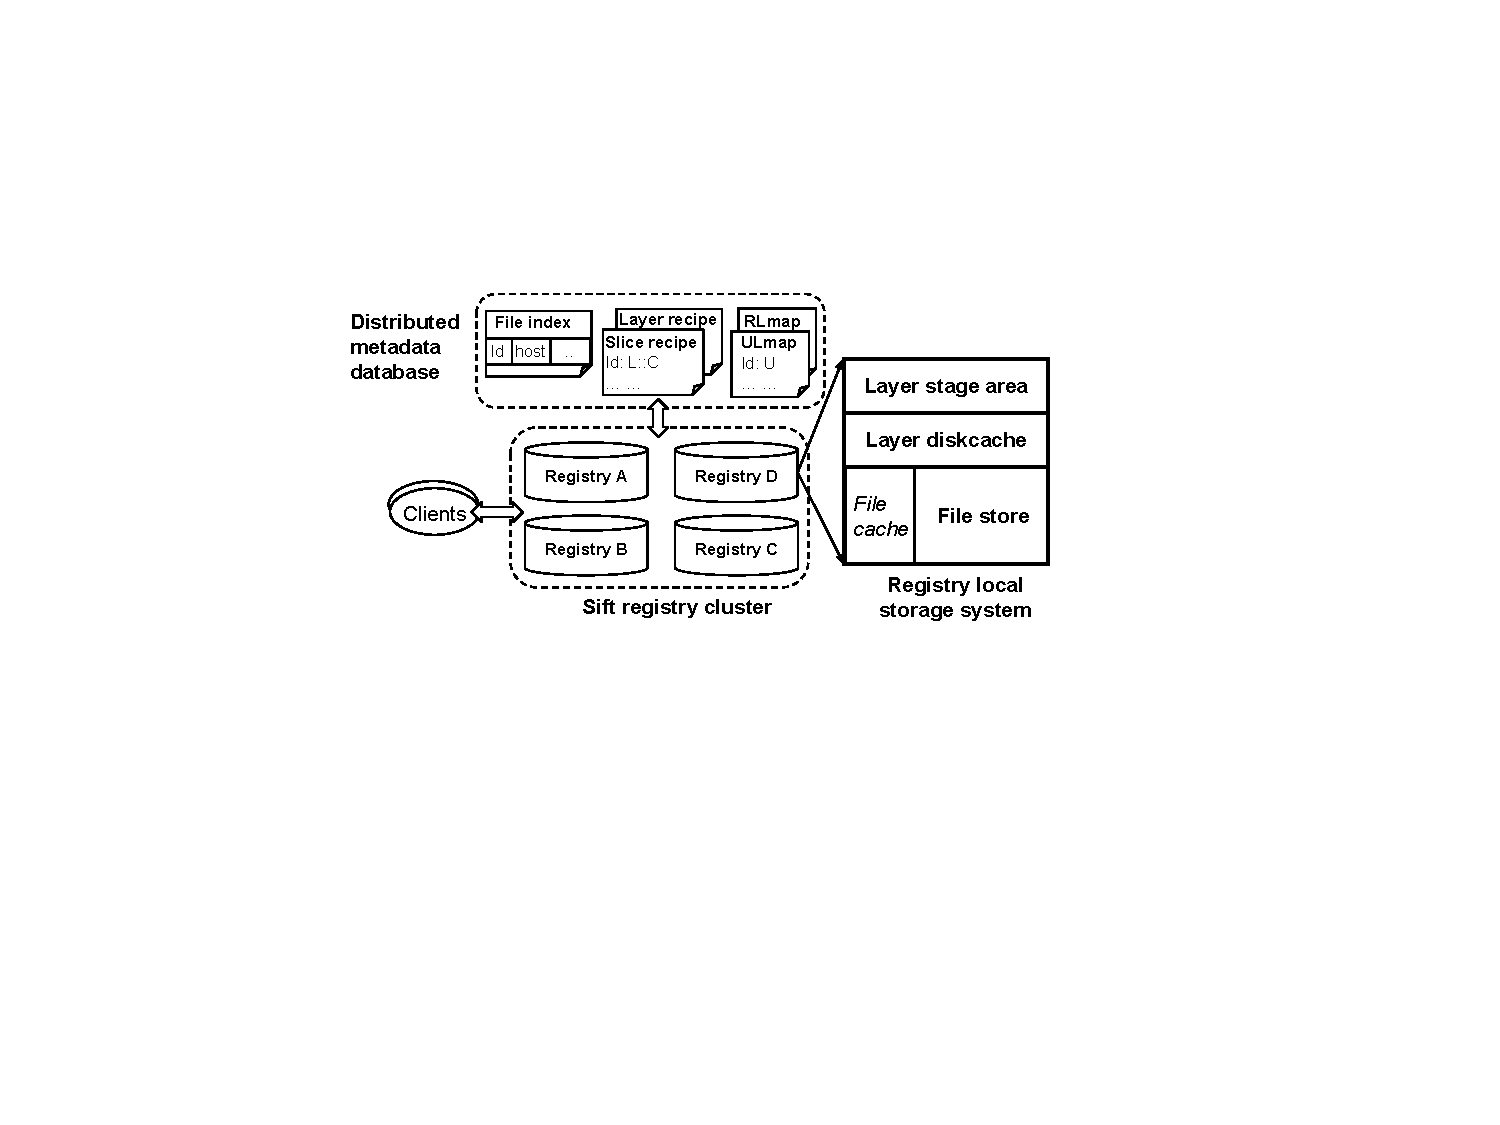
\includegraphics[width=0.9\textwidth]{graphs/sys-architecture.pdf}
%\vspace{-4pt}
			\caption{Architecture of \sysname.}
			%\label{fig:ref_count}
		%\end{minipage}
%	\begin{minipage}{0.225\textwidth}
%		\centering
%		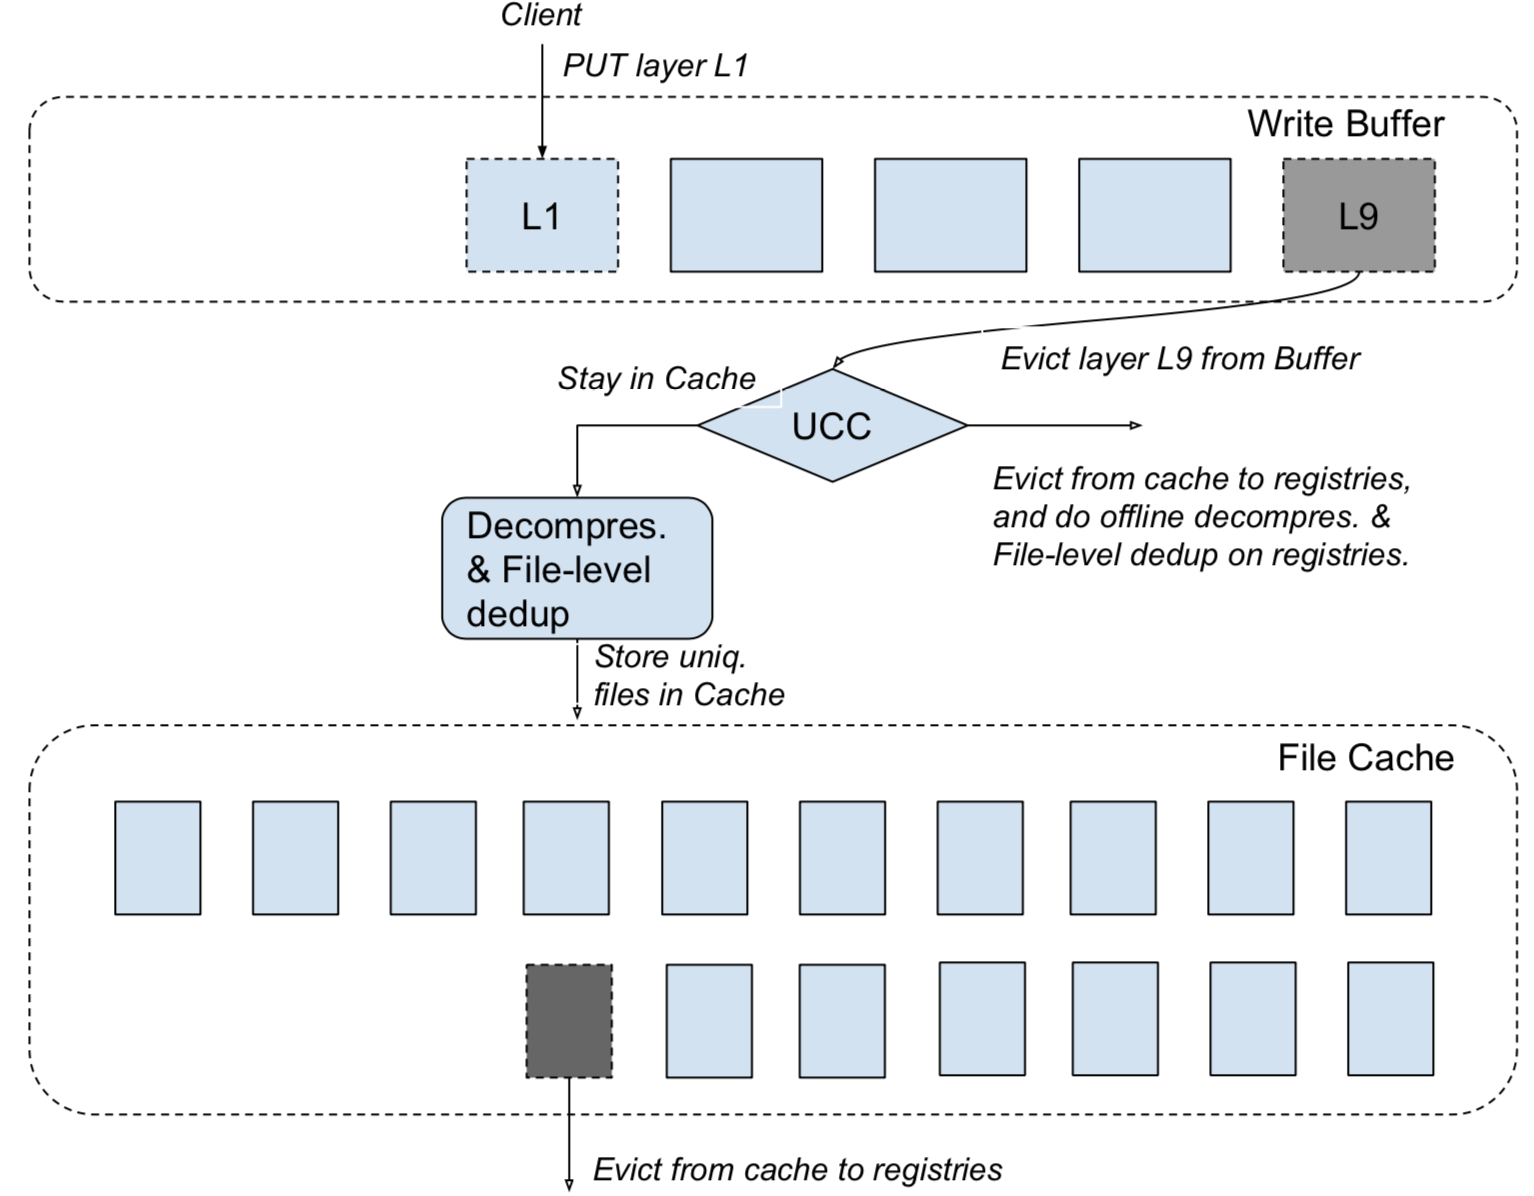
\includegraphics[width=1\textwidth]{graphs/slimmer-cache.png}
%		\caption{CDF of compress. and uncompress. layer size.}
%		\vspace{-3pt}
		\label{fig:sys-overview}
%\vspace{-4pt}
%	\end{minipage}
\end{figure*}

%\input{fig-diskcache}

\sysname provides different \emph{deduplication modes} by deduplicating different number of layer replicas
(see \ref{sec:dedup-mode}).
Figure~\ref{fig:sift-original} shows a simple deduplication mode of \sysname registry cluster compared with original registry cluster.
In the original registry cluster upon  a \texttt{push} request, 
registry \emph{A} stores the layer locally, denoted as \emph{primary layer replica}.
Meanwhile \emph{A} replicates the layer to other two servers: \emph{B} and \emph{C}, denoted as \emph{backup layer replicas}.
The subsequent \texttt{pull} layer requests can be served by any of the three layer replicas.
Similar to original registry cluster, 
\sysname first stores three layer replicas for newly \texttt{pushed} layers on three different servers: \emph{A}, \emph{B}, and \emph{C}. \emph{A} serves to store the primary layer replica, \emph{B} and \emph{C} store the backup layer replicas.
Then, one of the backup layer replicas (say, at server B) is \emph{deduplicated} into unique files, denoted as \emph{primary file replica}.
After that, each unique file is replicated and stored onto the remaining servers (in this case, \emph{C}), denoted as the \emph{backup file replicas}.
In the end, the two backup layer replicas at \emph{B} and \emph{C} are discarded while the primary layer replica at \emph{A} remains.
A \texttt{pull} layer request is first sent to registry \emph{A} which stores the primary layer replica.
If registry \emph{A} crashes,
Registry \emph{B} or \emph{C} can be used to reconstruct and serve the layer for the incoming \texttt{pull} layer request.
As a result, \sysname has the same level of redundancy as the original registry cluster. 

Figure~\ref{fig:sift} shows the architecture of \sysname.
 \sysname comprises a cluster of registry servers and a distributed metadata database. 
Registry servers store and serve both manifest and layer requests sent by clients.
Registry servers are divided into two groups:
\emph{primary cluster} and \emph{deduplication cluster}, denoted as \emph{P-servers} and \emph{D-servers}.
P-server mainly stores layer replicas and manifest replicas.
While D-server deduplicates the backup layer replicas at the file level and  stores replicates them.

As shown in Figure~\ref{fig:sift}, 
each D-server's local storage system is
divided into three parts: layer stage area, preconstruct cache, and file store. The \emph{Layer stage area} temporarily stores newly added layer replicas as shown in Figure~\ref{fig:sift-original}.
After a layer replica is \texttt{deduplicated}, 
the remaining unique files are stored as primary file replicas in a content 
addressable \emph{file store} with a small \emph{file cache}. 
Meanwhile, each unique file is replicated to the peer servers to provide redundancy.
The layer replica is then deleted from layer stage area.
To improve layer restoring performance, 
a layer replica is evenly divided into several \textbf{slices} and distributed across different registry servers so that
the layer can be restored in parallel (see section~\ref{sec:dedup-desgin}).
  
\emph{Preconstruct cache} on a D-server is an on-disk layer cache which contains preconstructed popular layers for later layer accesses to reduce latency in restoring (see section~\ref{sec:cache-design}).
%As shown in Figure~\ref{fig:cache}, 
When a P-server crashes,
the \texttt{pull} layer request will be served from a D-server.
If the \texttt{pull} layer request has a hit in the D-server's layer stage area (i.e. a layer replica has not been deleted yet),
the request will be served from layer stage area.

Upon a \texttt{pull} layer request miss, D-server will rebuild the layer from file store
based on its associated \textbf{layer recipe} (see section~\ref{sec:restore-design}). 
.
The preconstruct cache is a write-through cache; when layers are evicted from the diskcache, they are simply discarded.

Deduplication related metadata such as \textbf{layer recipe}, \textbf{slice recipe}, \textbf{layer index}, and \textbf{file index} is kept in a \emph{distributed database} (Figure~\ref{fig:sift}) for 
reliability, consistency, and fast accesses. 
Slice recipe and layer recipe are used to restore slices and rebuild layers.
Layer index and file index records \emph{content fingerprints} that are uniquely mapped to the associated physical layers and files respectively. %psychical file based on
Moreover, \sysname keeps track of user accesses and repository status, 
denoted as \textbf{ULmap} and \textbf{RLmap}, 
and saves them into the distributed metadata database.

In the following, we first describe different deduplication modes provided by \sysname.
Then, we describe how \sysname performs layer deduplication and layer restoring.

%\sysname uses a fast and reliable distributed database to 
%%, and unique files after layer deduplication
%The metadata such as layer recipes and slice recipes which
%Each server in the \sysname~registry cluster uses part of its storage for storing assembled (\ie preconstructed) layers. 
%We name such storage: user behavior based layer preconstruct cache (\preconstructcachename).
%Another part, a layer restoring performance--aware deduplication system (\dedupname system), is for storing deduplicated files. 
%Such files' metadata (\eg Docker image manifests) is kept in a metadata store; a distributed NoSQL database for 
%reliability, consistency, and fast accesses.
%
%

%\paragraph{Push}
%
%%As shown in Figure~\ref{fig:sys-overview}, 
%Consider a Docker client, client \textit{A}, who creates a new hello-world image
%\texttt{hello-world:new}
%from the official image which only contains a single layer \textit{L1}. 
%Pushing a new version of hello-world image corresponds to performing a PUT of layer \textit{L2} to the registry and a PUT of manifest to the metadata store as shown in Figure~\ref{fig:sys-overview}. 
%%first PUT
%Because the registry already stores \textit{L1}, 
%%only the modifications to the hello-world image that are commited as a new layer \textit{L2}, 
%only the compressed \textit{L2} tarball is PUT to the registry reflecting the modifications to the hello-world image.
%When \sysname~receives \textit{L2}, 
%it will cache \textit{L2} in the \preconstructcachename~for later accesses,
%and at the same time submit \textit{L2} to the backend storage system (Figure~\ref{fig:sys-overview}).
%The \preconstructcachename~uses write through policies. 
%Since layers are immutable, no data consistency issue exists between the \preconstructcachename~and the backend storage system.
%% Second PUT (manifest)
%The addition of layer \textit{L2} to the hello-world image is reflected in the manifest \textit{M1:0} which is PUT to the registry.
%Putting the new manifest \textit{M1:0} to the registry for the new image \texttt{hello-world:new} conlcudes the process of pushing it.
%
%
%
%The \dedupname~process runs periodically to deduplicate compressed layer tarballs (detailed in~\cref{sec:dedup-desgin})
%into unique files to save storage space.
%As shown in Figure~\ref{fig:sys-overview}, cold layer \textit{L2} is selected to be deduplicated.
%The \dedupname~process decompresses \textit{L2}, removes duplicate files from the \emph{uncompressed} \textit{L2}, and  evenly distributes the remaining unique files across the registry servers.
%This way, each server stores a 
%%\textbf{deduplicated slice}
%unique \textbf{slice}
% of the deduplicated \textit{L2}, from which a layer comprising a \textbf{slice} of \textit{L2}
%can be constructed and cached in the \preconstructcachename. We define such layer as a {\em slice layer}.
%We define all the per-server files belonging to a layer as a {\em deduplicated slice}. 
%Each server stores deduplicated slices belonging to many layers. 
%A layer is represented as a set of deduplicated slices that are distributed across multiple servers.
%The layer can be restored 
%%to a compressed layer tarball 
%from those distributed slices. 
%Such distribution allows restoring a layer in parallel.
%%To do that, 
%%\dedupname~process uses copy-on-write to update the old manifest \textit{M1:0} by adding slices' digests into it 
%%and generates new manifest \textit{M1:1} as shown in Figure~\ref{fig:sys-overview}.
%To do that, the \dedupname~process generates a new manifest \textit{M1:1} that holds, in addition to the contents of the old manifest \textit{M1:0}, the digests to the unique slices %comprising
%that make up the layer as shown in Figure~\ref{fig:sys-overview}.
%The slice digest is calculated by hashing the slice content~\cite{xxx}.
%
%\paragraph{Pull}
%
%As shown in Figure~\ref{fig:sys-overview},
%when client \textit{C} pulls an official image \texttt{hello-world} from the registry,
%\sysname~first checks if the requested layer \textit{L1} is present in~\preconstructcachename.
%If so, the \texttt{GET} layer request will be served by the cache.
%Otherwise, the \dedupname~system starts a parallel layer restoring process by serving slice layers from their hosting servers.
%For example, when client \textit{B} pulls the \texttt{hello-world:new} image from the registry,
%\sysname~sends the latest manifest (\textit{M1:1}) to client \textit{B}.
%After receiving \textit{M1:1}, client \textit{B} 
%%first 
%parses \textit{M1:1} to get a list of slice digests for \textit{L2}.
%Then, instead of sending a ``\texttt{GET layer L2}'' request, client \textit{B} will send multiple ``\texttt{GET slice of L2}'' requests to the registry.
%As shown in Figure~\ref{fig:sys-overview}, client \textit{B} sends ``\texttt{GET slice S1}'', ``\texttt{GET slice S2}'', and 
%``\texttt{GET slice S3}'' to the registry 
%since \textit{L2} is comprised of the slices \textit{S1}, \textit{S2}, and \textit{S3}.
%These requests are forwarded to the servers that store the corresponding deduplicated slice of \textit{L2}.
%%On \sysname~side, \textit{L2} is stored as deduplicated slices distributed across different servers.
%The servers will start to restore slices, \ie compose slice layers, from local deduplicated slices and send the compressed slices to the client 
%in parallel %as shown in Figure~\ref{fig:sys-overview}. 
%When client \textit{B} receives all the slices, it decompresses them together into an uncompressed layer.
%
%\paragraph{Docker client modifications}
% 
%To interact with \sysname, the Docker client is modified to 
%parse \sysname~manifests that include additional attributes, %-- 
%\ie slice digests.
%Also, if slice digests are present in a layer object in the manifest JSON file, 
%the client will replace ``\texttt{GET layer}'' request with multiple ``\texttt{GET slice}'' requests.
%Moreover, when the client receives the slices from registry, 
%the client decompresses these slices together into an uncompressed layer.  





%When a user requests a
%layer that is not present in the layer buffer, the request is forwarded to the
%file cache (detailed in~\cref{sec:design_operations}). 
%If a layer is also not found in the
%file cache, the request is forwarded to the backend dedup storage system.
%Note that after layer deduplication, unique files are
%scattered across multiple servers. 
%We define all the per-server files belonging to a layer as a {\em slice}. 
%A server stores slices for many layers, and a layer is composed of slices stored on multiple servers.
%To avoid the network latency caused by fetching slices from different servers and
%assembling them into a whole compressed layer, we split a \texttt{pull} request 
%into several~\texttt{pull slice}~requests. Those requests will then be
%forwarded to all the backend servers that store the requested
%layer's slices. 
%After a~\texttt{pull slice}~request is received, each backend server compresses the slice 
%and directly sends it back to the user.
%We modify the Docker client
%interface such that when it receives all the compressed slices, it can
%decompress them into a single layer. 
%Furthermore, compressing slices in parallel considerably lowers the layer compression latency,
%since compression time depends on the size of the
%uncompressed data.
%to cache layers and cache unique files after decompression and deduplication,
%respectively.  consists of a \emph{layer buffer} and a \emph{file cache}.  The
%layer buffer stores all the newly pushed layers in memory.  Although accessing
%memory is very fast, the size of main memory is limited. 
%All the slices for a layer are fetched in parallel for performance improvement.






%\sysname~seamlessly integrates 
%%the management of 
%caching and deduplication on the
%backend storage system (\emph{backend dedup storage}) with Docker registries.
%%
%We address a set of unique challenges to enable this integration.
%%
%First, for caching layers, \texttt{pull} layer requests are difficult to
%predict because layers are accessed infrequently.
%In~\cref{sec:background},
%%\arb{???}, 
%we have observed that about half of the layers are not
%accessed again for at least $1.3$~hours. Which means that if we
%cache a layer, we may need to wait a long time before we observe a hit on that layer.  %(as discussed in~\cref{sec:background}).  
%This is mainly 
%because when a user pulls an image from the registry, the Docker daemon on the
%requesting host will only pull the layers that are not locally stored.
%%\Ali{I do not understand the following sentence.}
%%Moreover, we have to consider that a user might deploy an applications on
%%multiple machines, so it's not easy to predict when a user will access which layers. 
%%%\Ali{The above statement is incorrect. You have to distinguish between GET layer requests
%%that are issued after a (PUSH layer + GET manifest) request and a normal GET layer request.
%%FAST paper only talk about case 1. Whereas you are generalizing that any GET layer request
%%should have a precedent GET layer request which is wrong. We can make a case
%%that not all GET layers requests have a precedent PUSH layer request but we can
%%not say that it takes a few days, weeks, or even months for a user to make a pull
%%layer request after a push layer request.}
%%\NZ{I mean the first case, push beyond your trace collection time.}
%%
%
%Second, we can not deduplicate compressed layers. For deduplication, each layer
%needs to be uncompressed, and only then can undergo file-level deduplication. Similarly,
%to restore a layer, we need to fetch files from multiple servers, and only then compress
%them in to a tar file to serve a \texttt{pull} layer request. 
%%\arb{that can service the ??? request}\NZ{addressed}. 
%This whole process can incur a 
%considerable performance overhead on \texttt{pull} layer requests.
%Deduplication also slows down
%\texttt{push} layer requests because of its high demand for CPU, memory, I/O, and network resources.
%%\Ali{Explain how push layer requests are not effected?}\NZ{fixed}
%
%%\subsection{Design}
%To address these issues, we propose a new registry design. The key feature of our design is a user-access-history-based prefetch algorithm that helps mitigate the performance degradation due to the 
%backend dedup storage system (Figure~\ref{fig:sys-overview}). Based
%on layer access pattern we observed in~\cref{sec:background} and user access history information,
%\sysname precisely prefetch the layers that may be pulled shortly.
%%has not been pulled in the requested repository
%%and the prefetched 
%%In this case, we can   
%%a user's active time is predictable. 
%%Thus, we leverage users' behavior, \ie
%%when a user is most likely to be active, to drive layer evictions from the cache.
%
%
%%\begin{figure}[t]
	\centering
		%\begin{minipage}{0.225\textwidth}
			\centering
			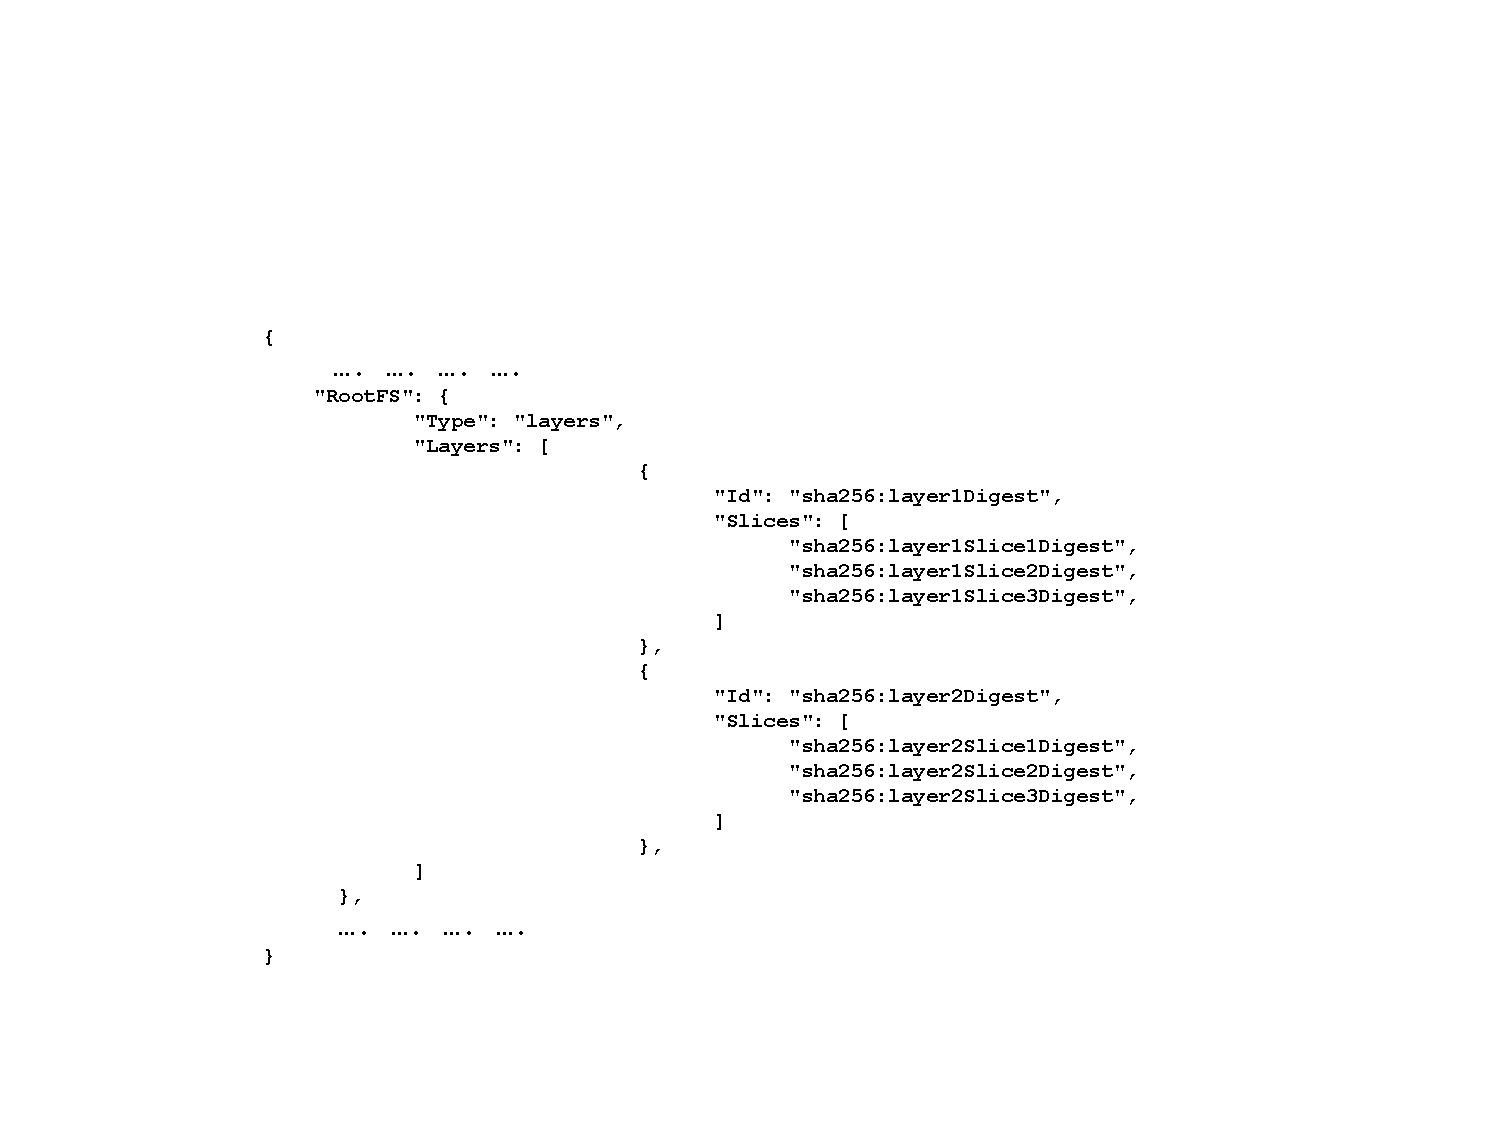
\includegraphics[width=0.4\textwidth]{graphs/fig-sift-manifest}
%\vspace{-4pt}
			\caption{\sysname~manifest.}
			%\label{fig:ref_count}
		%\end{minipage}
%	\begin{minipage}{0.225\textwidth}
%		\centering
%		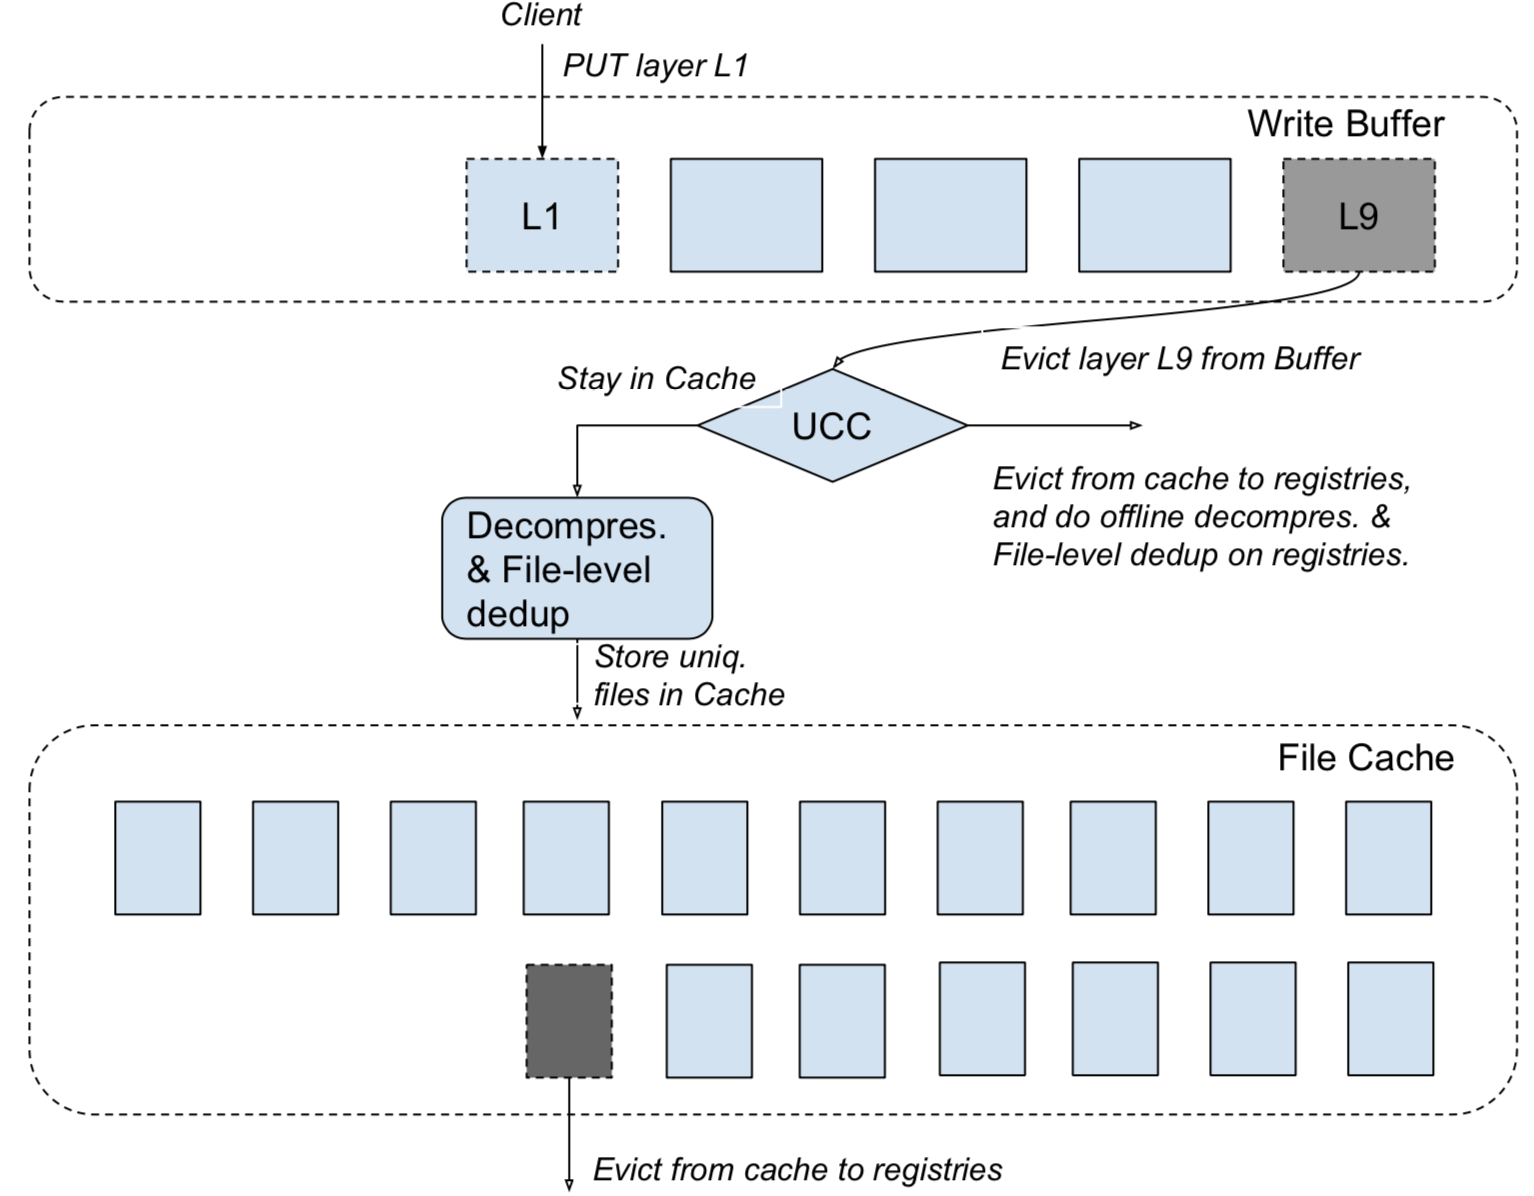
\includegraphics[width=1\textwidth]{graphs/slimmer-cache.png}
%		\caption{CDF of compress. and uncompress. layer size.}
%		\vspace{-3pt}
		\label{fig:sys-overview}
%\vspace{-4pt}
%	\end{minipage}
\end{figure}
%
%Considering that layer sizes are typically about several MB~\cite{dockerworkload}, 
%a small main memory cache will be unable to accommodate
%all prefetched layers for all active users. 
%To address this issue, we 
%create separate caches for layers and \emph{unique} files, called {\em layer buffer} and {\em file cache}, respectively. 
%%Both caches comprise both
%%main memory and flash memory.
%%Layer buffer
%%\arb{are main memory for one type and flash for the other type, or both for both types. I assumed both types of memory are used, and there are two caches. check previous sentence for correctness.}\NZ{addressed}
%Note that, layers are  compressed tarballs and buffered in layer buffer, and 
%%sent by users
% \emph{unique} files are uncompressed files from which duplicates have been removed and stored on flash-based storage. 
%%We call compressed layer cache and \emph{deduped} files cache,
%%\emph{layer buffer} and \emph{file cache}, respectively.
%For 
%cache evictions, we first evict inactive users' layers from the layer buffer.
%Next, we \emph{dedup} the evicted layers, then store the \emph{unique} files
%into the file cache (detailed in~\cref{sec:design_operations}). 
%%the following operations: decompressing each evicted layer and comparing its
%%containing files with the files that are already stored in the file cache,
%%eliminating duplicate files, that is, only storing the unique files on flash
%%storage.



 
